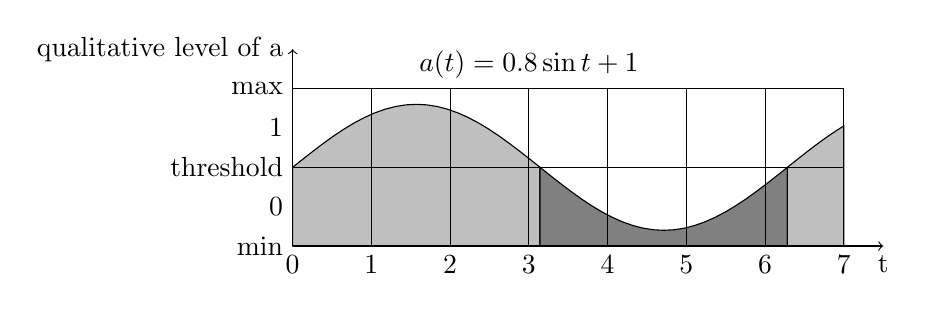
\begin{tikzpicture}
\draw[->] (0,0) -- (0,2.5);
\draw[->] (0,0) -- (7.5,0);
\draw(0,2)node[left]{max};
\draw(0,0)node[left]{min};
\draw(0,1)node[left]{threshold};
\foreach \y in {0,1} \draw(0,\y+0.5)node[left]{\y};
\foreach \x in {0,1,...,7} \draw(\x,0)node[below]{\x};
\filldraw[draw=black,fill=black!25!white]
	plot[domain=0:pi] (\x, {0.8*sin(\x r)+1})--(pi,0)--(0,0)--(0,1); 
\filldraw[draw=black,fill=gray]
	plot[domain=pi:2*pi] (\x, {0.8*sin(\x r)+1})--(2*pi,0)--(pi,0)--(pi,1); 
\filldraw[draw=black,fill=black!25!white]
	plot[domain=2*pi:7] (\x, {0.8*sin(\x r)+1})--(7,0)--(2*pi,0)--(2*pi,1); 
\draw[step=1] (0,0) grid (7,2);
\draw (7.5,0) node[below]{t};
\draw (0,2.5) node[left]{qualitative level of a};
\draw(3,2)node[above]{$a(t)=0.8\sin t+1$};
\end{tikzpicture}